
%%% use twocolumn and 10pt options with the asme2e format
\documentclass[twocolumn,10pt, final]{asme2e}
\addtolength{\textwidth}{-1pt}

\usepackage{cite}
\usepackage[pdftex]{graphicx}
\usepackage[cmex10]{amsmath}
\usepackage{amssymb}
\usepackage{algpseudocode}
\usepackage{array}
\usepackage{tikz}
\newcommand*\circled[1]{\tikz[baseline=(char.base)]{
            \node[shape=circle,draw,inner sep=2pt] (char) {#1};}}
\hyphenation{REFERENCE}

%% The class has several options
%  onecolumn/twocolumn - format for one or two columns per page
%  10pt/11pt/12pt - use 10, 11, or 12 point font
%  oneside/twoside - format for oneside/twosided printing
%  final/draft - format for final/draft copy
%  cleanfoot - take out copyright info in footer leave page number
%  cleanhead - take out the conference banner on the title page
%  titlepage/notitlepage - put in titlepage or leave out titlepage
%  
%% The default is oneside, onecolumn, 10pt, final

%%% Replace here with information related to your conference
\conffullname{Proceedings of the ASME 2015 Dynamic Systems and Control Conference}
\confshortname{DSCC2015}
\confdate{28-30}
\confmonth{October}
%%%%% for date across two months, use
%\confdate{October 31-November 3}
%%%%\confmonth{September}
\confyear{2015 }
\confcity{Columbus, Ohio}
\confcountry{USA}

%%% Replace DETC2005-12345 with the number supplied to you 
%%% by ASME for your paper.
\papernum{DSCC2015-9757}

\title{A Sequential Two-Step Algorithm for Fast Generation of Vehicle Racing Trajectories}

%%% first author
\author{Nitin R. Kapania \thanks{Address all correspondence to this author.}
    \affiliation{
	School of Mechanical Engineering\\
	Stanford University\\
	Stanford, CA 94305\\
	nkapania@stanford.edu
    }	
}

%%% second author
%%% remove the following entry for single author papers
%%% add more entries for additional authors
\author{John Subosits
    \affiliation{School of Mechanical Engineering\\
	Stanford University\\
	Stanford, CA 94305\\
	subosits@stanford.edu
    }
}

\author{J. Christian Gerdes
    \affiliation{School of Mechanical Engineering\\
	Stanford University\\
	Stanford, CA 94305\\
	gerdes@stanford.edu
    }
}

\begin{document}

\maketitle    

%%%%%%%%%%%%%%%%%%%%%%%%%%%%%%%%%%%%%%%%%%%%%%%%%%%%%%%%%%%%%%%%%%%%%%
\begin{abstract}
{\it The problem of maneuvering a vehicle through a race course in minimum time requires computation of 
 both longitudinal (brake and throttle) and lateral (steering wheel) control inputs.    
 Unfortunately, solving the resulting nonlinear optimal control problem is typically computationally expensive and infeasible for real-time trajectory planning.
 This paper presents an iterative algorithm that divides the path generation
 task into two sequential subproblems that are significantly easier to solve. Given an initial path through the race track, the algorithm
 runs a forward-backward integration scheme to determine the minimum-time longitudinal speed profile, subject to
 tire friction constraints. With this speed profile fixed, the algorithm updates the vehicle's path by solving a convex optimization problem 
 that minimizes the resulting path curvature while staying within track boundaries and obeying affine, time-varying vehicle dynamics constraints.
 This two-step process is repeated iteratively until the
 predicted lap time no longer improves. While providing no guarantees of convergence or a globally optimal solution, 
 the approach performs well when tested on the Thunderhill Raceway
 course in Willows, CA. The lap time reaches a minimum value after only three iterations, with each iteration over the full 5 km race course requiring
 only thirty seconds of computation time on a laptop computer. The resulting vehicle path and speed profile match very well with a nonlinear gradient
 descent solution and a path driven by a professional racecar driver, indicating that the proposed method is a viable option for online trajectory
 planning in the near future.}
\end{abstract}

%%%%%%%%%%%%%%%%%%%%%%%%%%%%%%%%%%%%%%%%%%%%%%%%%%%%%%%%%%%%%%%%%%%%%%
\section*{INTRODUCTION}

The problem of calculating the minimum lap time trajectory for a given vehicle and race track has been studied over the last several decades
in the control, optimization, and vehicle dynamics communities.  Early research by Hendrikx et al.. \cite{hendrikx} in 1996 used 
 Pontryagin's minimum principle to derive coupled differential equations to solve for the minimum-time trajectory
for a vehicle lane change maneuver. The minimum lap time problem drew significant interest from professional racing teams, and
Casanova \cite{casanova} published a method in 2000 capable of simultaneously optimizing both the path and speed profile
for a fully nonlinear vehicle model using nonlinear programming (NLP). Kelley \cite{kelly} further extended the results from Casanova to 
consider transient vehicle dynamics and tire thermodynamics. 

More recently, the development of autonomous vehicle technology at the industry and academic level has led to research on optimal path
 planning algorithms that can be used for driverless cars. Theodosis and Gerdes published a gradient descent approach for determining time-optimal
  racing lines, with the racing line constrained to be composed of a fixed number of clothoid segments \cite{theodosis}. Given the computational expense
 of performing nonlinear optimization, there has also been a significant research effort to find approximate methods that provide fast lap times.
 Timings and Cole \cite{timings} formulated the minimum lap time problem into a model predictive control (MPC) problem by linearizing the nonlinear vehicle
 dynamics at every time step and approximating the minimum time objective by maximizing distance traveled along the path centerline. Gerdts et al. 
 \cite{gerdts} proposed a similar receding horizon approach, where distance along a reference path was maximized over a series of locally optimal optimization
 problems that were combined with continuity boundary conditions. One potential drawback of the model predictive control approach is that an optimization
 problem must be reformulated and solved at every time step, which can still be computationally expensive. For example, Timings and Cole reported a computation time of 920 milliseconds
 per 20 millisecond simulation step on a desktop PC.
 
 In general, the aforementioned methods are still feasible for experimental implementation. As demonstrated in \cite{mickgeneral}, 
 an autonomous vehicle  can apply a closed-loop controller to follow a time-optimal vehicle trajectory computed offline. However, there are
 significant benefits to developing a fast trajectory generation algorithm that can approximate the globally optimal trajectory.
 If the algorithm runtime is small compared to the actual lap time, the algorithm can run as a real-time trajectory planner and find a fast racing line 
 for the next several turns of the racing circuit. This would allow the trajectory planner to modify the desired path based on estimates of
 road friction, tire wear, engine/brake dynamics and other parameters learned over several laps of racing. Additionally, the fast trajectory algorithm can
 be used to provide a very good initial trajectory for a nonlinear optimization method.  
  
 This paper therefore presents an iterative algorithm that generates vehicle racing trajectories with low computational expense. 
 To speed up computation time, the combined lateral/longitudinal optimal control problem is replaced by two sequential sub-problems 
 where minimum-time longitudinal speed inputs are computed given a fixed vehicle path, and then the vehicle path is updated given the fixed speed commands. The following section presents a mathematical framework for the overall trajectory generation
 problem and provides a linearized five-state model for the planar dynamics of a racecar following a set of speed and steering inputs, with lateral and heading error states computed with respect to a fixed path.
 The next section describes the method of finding the minimum time speed inputs given a fixed path.  While this sub-problem has been recently formulated as a convex optimization problem \cite{lipp}, a forward-backward
 integration scheme based on prior work \cite{subosits} is used instead.  Next, the paper describes a method for updating the racing path given the fixed speed inputs using convex optimization, where the curvature norm
 of the driven path is explicitly minimized. The last section presents the final algorithm and compares results generated on the Thunderhill Raceway circuit
 in Willows, CA to results from both a nonlinear optimization and data recorded from a professional racecar driver. The paper concludes by discussing 
 future implementation of the algorithm in a real-time path planner.  
\\\\
%%%%%%%%%%%%%%%%%%%%%%%%%%%%%%%%%%%%%%%%%%%%%%%%%%%%%%%%%%%%%%%%%%%%%%
\section*{PATH DESCRIPTION AND VEHICLE MODEL}

Figure~\ref{fig:worldInfo} describes the parameterization of the reference path that the vehicle will follow. The reference path is most intuitively described in Fig.~\ref{fig:worldInfo}a as a 
smooth curve of Cartesian East-North coordinates, with road boundaries represented by similar Cartesian curves. However, for the purposes of quickly generating
a racing trajectory, it is more convenient to parameterize the reference path as a curvature profile $K$ that is a function of distance along the path $s$ (Fig.~\ref{fig:worldInfo}c). Additionally, it is 
convenient to store the road boundary information as two functions $w_\mathrm{in}(s)$ and $w_\mathrm{out}(s)$, which correspond to the lateral distance from the path at $s$
 to the inside and outside road boundaries, respectively (Fig.~\ref{fig:worldInfo}b). This maximum lateral distance representation will be useful when constraining the generated racing path to lie within the road 
 boundaries. The transformation from the local $s$, $K$ coordinate frame to 
the global Cartesian coordinates $E$, $N$ are given by the Fresnel integrals:
\begin{figure}
\centering
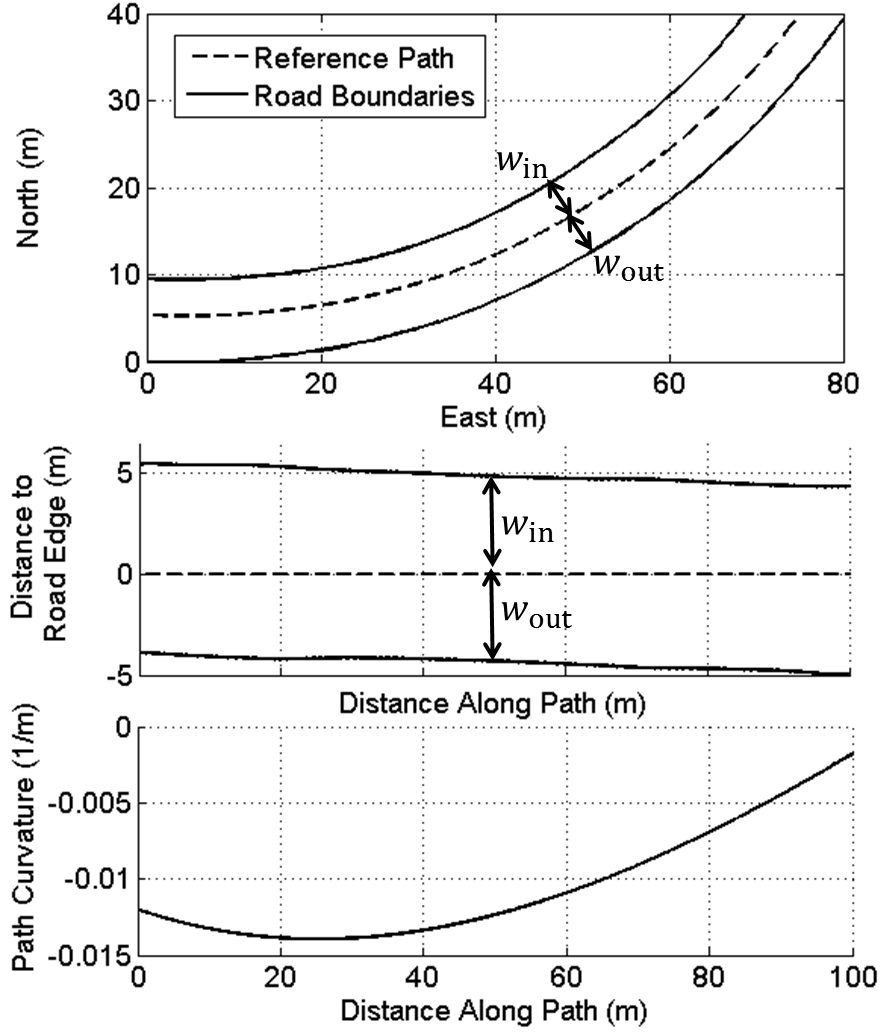
\includegraphics[width=3.5in]{figures/worldInfo.png}
\caption{(a) View of a sample reference path and road boundaries, plotted in the East-North Cartesian frame (b) Lateral distance from path to inside road edge (positive) and outside road edge (negative) as a function
of distance along path. (c) Curvature as a function of distance along path.}
\label{fig:worldInfo}
\end{figure}
\begin{subequations}
\label{eq:fresnel}
\begin{align}
	E(s) &= \int_0^s  -\sin(\Psi_\mathrm{r}(z)) dz \\
	N(s) &= \int_0^s   \cos(\Psi_\mathrm{r}(z)) dz \\
	\Psi_\mathrm{r}(s) &= \int_0^s K(z) dz \label{eq:balls}
\end{align}
\end{subequations}
where $\Psi_\mathrm{r}(s)$ is the heading angle of the reference path. With the reference path defined in terms of $s$ and $K$, the 
next step is to define the dynamic model of the vehicle. For the purposes of trajectory generation, we assume the vehicle dynamics are given 
by the planar bicycle model (Fig.~\ref{fig:bikemodel}a), with yaw rate $r$ and sideslip $\beta$ states describing the lateral dynamics. Additionally, the vehicle's offset from
the reference path is given by the path lateral deviation state $e$ and path heading error state $\Delta\Psi$ (Fig.~\ref{fig:bikemodel}b). Equations of
motion for all four states are given by:
\begin{subequations}
\label{eq:bm}
\begin{align}
	\dot{\beta} &= \frac{F_\mathrm{yf}+F_\mathrm{yr}}{mU_\mathrm{x}(t)} - r \qquad \dot{r} = \frac{aF_\mathrm{yf} - bF_\mathrm{yr}}{I_z} \label{bm1} \\
	\dot{e} &= U_\mathrm{x} (\beta + \Delta\Psi) \qquad \Delta\dot{\Psi} = r - U_\mathrm{x}K \label{eq:bm2} 
\end{align}
\end{subequations}
where $U_\mathrm{x}$ is the vehicle forward velocity and $F_\mathrm{yf}$ and $F_\mathrm{yr}$ are the front and rear lateral tire forces. 
The vehicle mass and yaw inertia are denoted by $m$ and $I_z$, and the geometric parameters $a$ and $b$ are shown in Fig.~\ref{fig:bikemodel}a. Note
that while the vehicle longitudinal dynamics are not explicitly modeled, the bicycle model does allow for time-varying values of $U_\mathrm{x}$. 
\begin{figure}
\centering
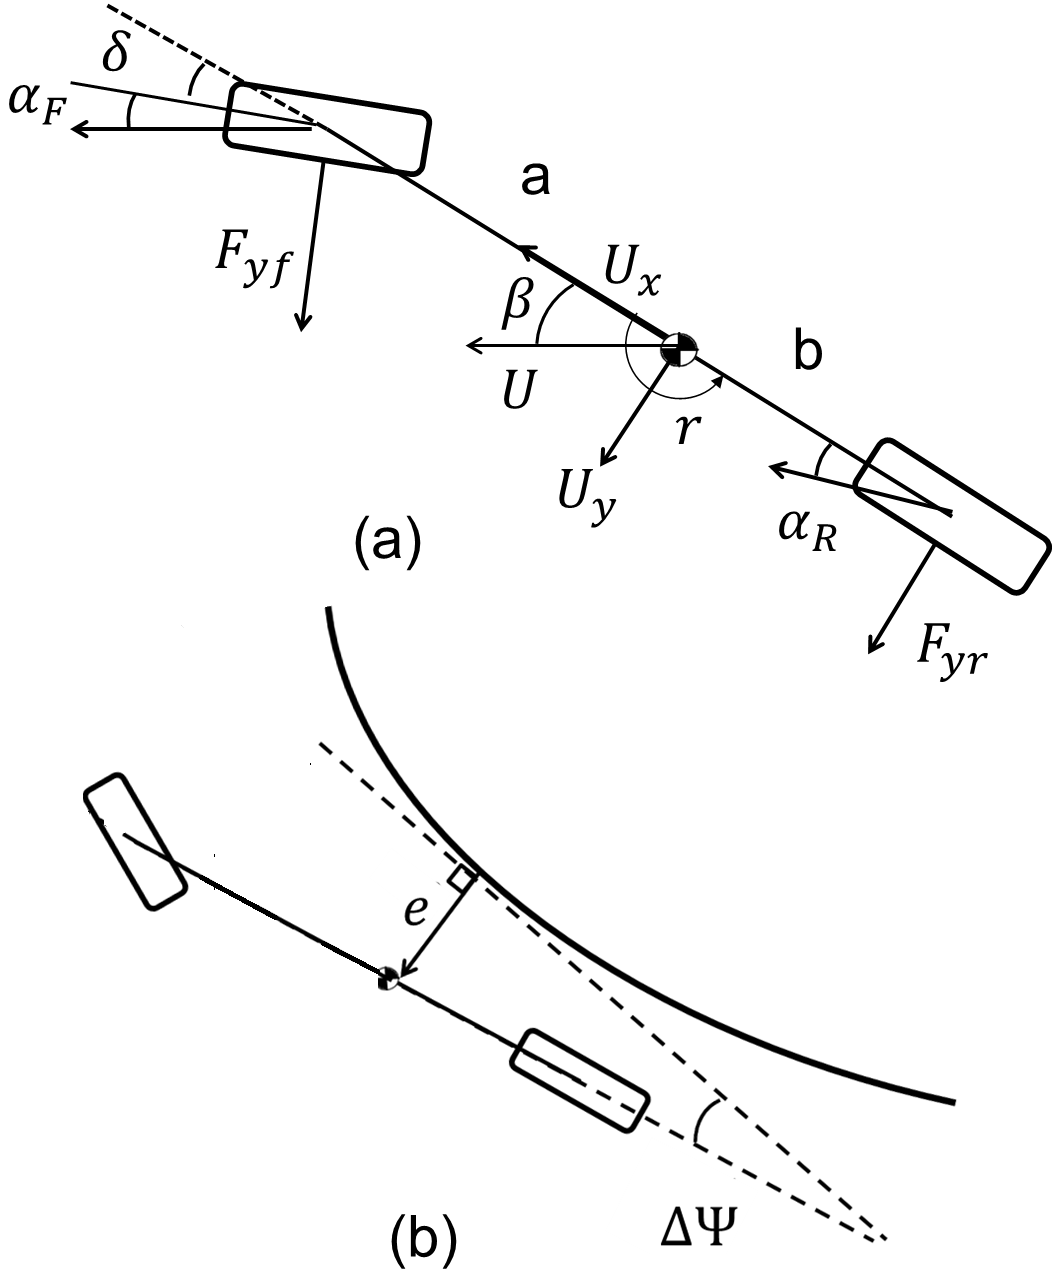
\includegraphics[width=2.5in]{figures/BikeModelSchematic.png}
\caption{(a) Schematic of bicycle model. (b) Diagram showing lateral path deviation $e$ and path heading error $\Delta\Psi$ states.}
\label{fig:bikemodel}
\end{figure}


%%%%%%%%%%%%%%%%%%%%%%%%%%%%%%%%%%%%%%%%%%%%%%%%%%%%%%%%%%%%%%%%%%%%%%
\section*{VELOCITY PROFILE GENERATION GIVEN FIXED REFERENCE PATH}
Given a fixed reference path described by $s$ and $K$, the first algorithm step is to find the minimum time speed profile the vehicle can achieve
without exceeding the available tire-road friction. The approach taken in this paper is a ``three-pass" approach described in complete detail by 
Subosits and Gerdes \cite{subosits}, and originally inspired by work from Velenis et al.. \cite{velenis}. 
Given the lumped front and rear tires from Fig.~\ref{fig:bikemodel}a, the available longitudinal
force $F_\mathrm{x}$ and lateral force $F_\mathrm{y}$ at each wheel is given by the friction circle constraint: 
\begin{subequations}
\label{eq:tireforce}
\begin{align}
	F^2_\mathrm{xf} + F_\mathrm{yf}^2 &\leq (\mu F_\mathrm{zf})^2\\
	F^2_\mathrm{xr} + F_\mathrm{yr}^2 &\leq (\mu F_\mathrm{zr})^2
\end{align}
\end{subequations}
where $\mu$ is the tire-road friction coefficient and $F_\mathrm{z}$ is the available normal force at the tire. The method described in \cite{subosits} 
determines the normal and lateral tire forces $F_\mathrm{z}$ and $F_\mathrm{y}$ at each point along the path 
by accounting for factors such as longitudinal weight transfer and three-dimensional 
topography effects (e.g. road bank and grade). However, for this paper, we will consider only the primary
effects of road curvature, vehicle speed, and static weight distribution. The first pass of the speed profile generation aims to find the maximum permissible steady state vehicle speed given zero longitudinal force. This is given
by:
\begin{equation}
\label{eq:steadystate}
	U_\mathrm{x}(s) = \sqrt{\frac{\mu g}{|K(s)|}}
\end{equation}
where the result in (\ref{eq:steadystate}) is obtained by setting $F_\mathrm{yf} = \frac{mb}{a+b}U_\mathrm{x}^2K$ and $F_\mathrm{zf} = \frac{mgb}{a+b}$.
 The results of this first pass for the sample curvature profile in Fig.~\ref{fig:VPgen}a are shown in Fig.~\ref{fig:VPgen}b.
 The next step is a forward 
integration step, where the velocity of a given point is determined by the velocity of the previous point and the available longitudinal force $F_{x,\mathrm{max}}$ for acceleration.
This available longitudinal force is calculated in \cite{subosits} by accounting for the vehicle engine force limit and the lateral force demand on all tires due to the road curvature:
\begin{equation}
\label{eq:forwardint}
	U_x(s+\Delta s) =\sqrt{U_x(s)+\mathrm{2}\frac{F_{x,\mathrm{accel,max}}}{m}\Delta s}
\end{equation}
A key point of the forward integration step is that at every point, the value of $U_\mathrm{x}(s)$ is compared to the corresponding value from (\ref{eq:steadystate}), and
the minimum value is taken. The result is shown graphically in Fig.~\ref{fig:VPgen}c. Finally, the backward integration step occurs, where the available
longitudinal force for deceleration is constrained by the lateral force demand at both tires:
\begin{equation}
\label{eq:backwardsint}
	U_x(s-\Delta s) = \sqrt{U_x(s)-\mathrm{2}\frac{F_{x,\mathrm{decel,max}}}{m}\Delta s}
\end{equation}
The value of $U_\mathrm{x}(s)$ is then compared to the corresponding value from (\ref{eq:forwardint}) for each point along the path, and the minimum
value is chosen, resulting in the final velocity profile shown by the solid line in Fig.~\ref{fig:VPgen}d. 
 \begin{figure}
\centering
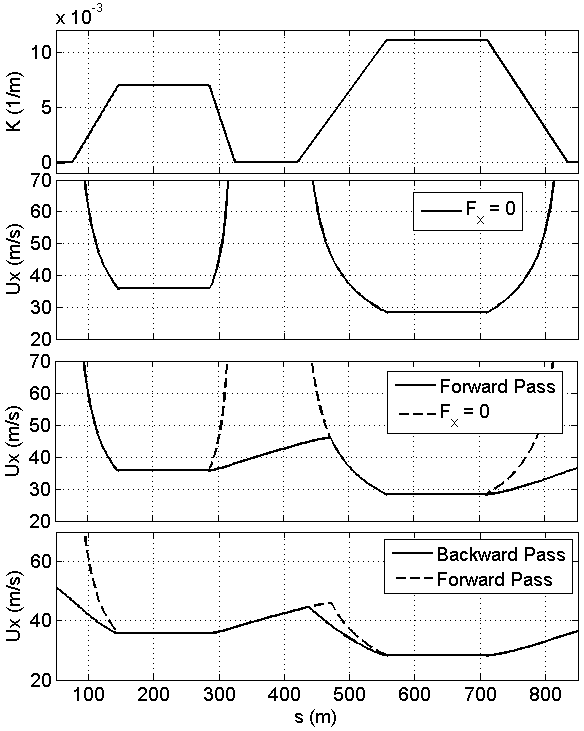
\includegraphics[width=3.5in]{figures/vpgen.png}
\caption{(a) Sample curvature profile. (b) Velocity profile given zero longitudinal force. (c) Velocity profile after forward pass (d) Final velocity profile after backward pass. }
\label{fig:VPgen}
\end{figure}


%%%%%%%%%%%%%%%%%%%%%%%%%%%%%%%%%%%%%%%%%%%%%%%%%%%%%%%%%%%%%%%%%%%%%%
\section*{UPDATING PATH GIVEN FIXED VELOCITY PROFILE}
\subsection*{Overall Approach and Minimum Curvature Heuristic}
The second step of the trajectory generation algorithm takes the original reference path $K(s)$ and corresponding velocity profile $U_x(s)$
as inputs, and modifies the reference path to obtain a new, ideally faster, racing line. Sharp \cite{sharp} suggests a general approach for modifying 
an initial path to obtain a faster lap time by taking the original path and velocity profile and incrementing the speed uniformly
by a small, constant ``learning rate." An optimization problem is then solved to find a new reference path and control inputs that allow the vehicle to
drive at the higher speeds without driving off the road. If a crash is detected, the speed inputs are locally reduced around the crash site and the process is repeated.

However, one challenge with this approach is that it can take several hundred iterations of locally modifying the vehicle speed profile, detecting crashes, and 
 modifying the reference path to converge to a fast lap time. An alternative approach is to minimize
 the norm of the vehicle curvature $K(s)$ at each path modification step. Intuitively, as the speed profile increases,
 the reference path will need to be modified to have lower peak curvature values in order to avoid saturating the lateral force capabilities of the tire.
 However, the minimum curvature path is not, in general, the minimum time path. In general, the minimum time path must tradeoff between the competing objectives of minimizing the path curvature to increase cornering speed,
while also shortening the overall length of the path.
\subsection*{Convex Problem Formulation}
Formulating the path update step as a convex optimization problem requires an affine, discretized form of the
bicycle model presented earlier. The equations of motion in (\ref{eq:bm}) are already linearized, but
 the front and rear lateral tire forces become saturated as the vehicle drives near the limits of tire adhesion. 
The well-known brush tire model \cite{Pacejka2012} captures the force saturation of tires as a function of lateral tire slip angle $\alpha$ as follows:
\small
\begin{eqnarray}
\label{eq:fiala}
	F_\mathrm{y\star}&=&\begin{cases} -C_{\star}\tan\alpha_\star + \frac{C_\star^2}{3\mu F_\mathrm{z\star}} |\tan\alpha_\star| \tan\alpha_\star \\ \hspace{10mm}- \frac{C_\star^3}{27\mu^2F_\mathrm{z\star}^2}\tan^3\alpha_\star,
\hspace{8mm}  |\alpha_\star| < \arctan{\left(\frac{3\mu F_\mathrm{z\star}}{C_\star}\right)} \\ \\ -\mu F_\mathrm{z\star}\text{sgn} \ \alpha_\star, \hspace{36mm} \mathrm{otherwise} \end{cases}
\end{eqnarray}
\normalsize
where the symbol $\star \in [\mathrm{f},\mathrm{r}]$ denotes the lumped front or rear tire, and $C_\star$ is the corresponding tire cornering stiffness. 
The linearized tire slip angles $\alpha_\mathrm{f}$ and $\alpha_\mathrm{r}$ are functions of the vehicle lateral states and the steer angle
input, $\delta$:
\begin{subequations}
\begin{align}
	\alpha_\mathrm{f} &= \beta + \frac{ar}{U_\mathrm{x}} - \delta\\
	\alpha_\mathrm{r} &= \beta - \frac{br}{U_\mathrm{x}}
\end{align}
\end{subequations}
 \begin{figure}
\centering
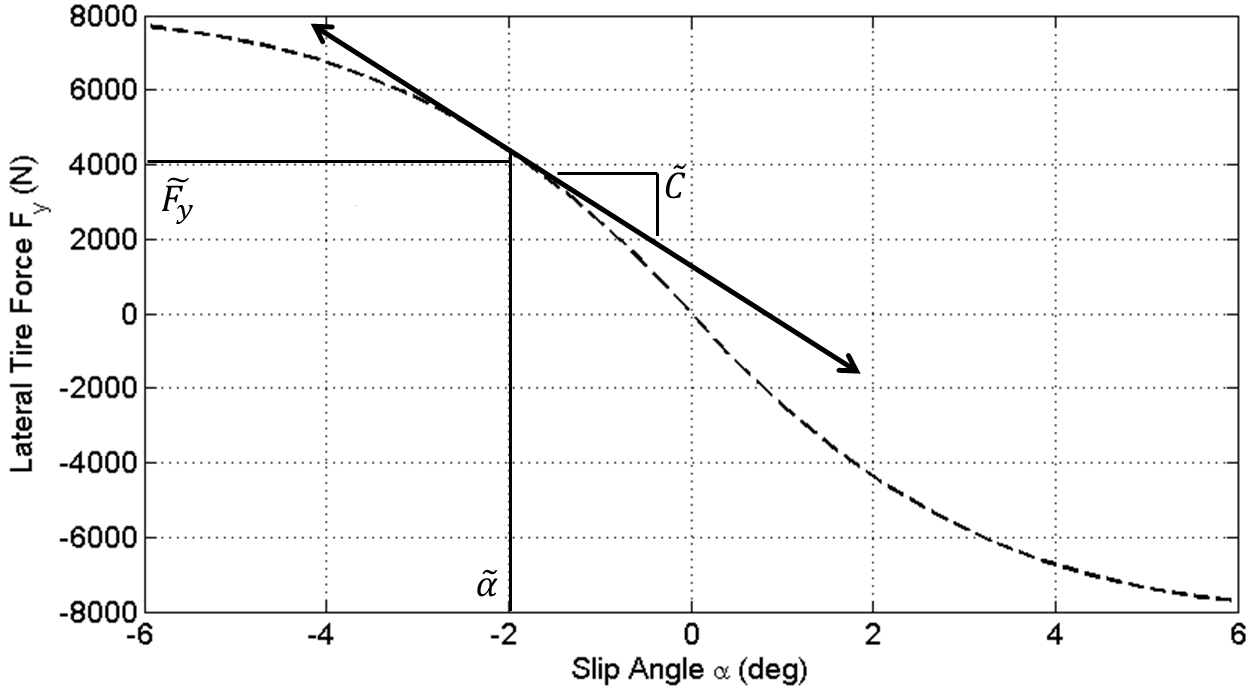
\includegraphics[width=3.5in]{figures/fiala.png}
\caption{Nonlinear tire force curve given by Fiala model, along with affine tire model linearized at $\alpha = \tilde{\alpha}$. }
\label{fig:fiala}
\end{figure}
The brush tire model in (\ref{eq:fiala}) can be linearized at every point along the reference path assuming steady state cornering conditions:
\begin{subequations}
\begin{align}
	F_\mathrm{y\star} &= \tilde{F}_\mathrm{y\star} - \tilde{C}_\star(\alpha_\star - \tilde{\alpha}_\star) \\
	\tilde{F}_\mathrm{y\star} &= \frac{F_\mathrm{z\star}}{g} U_\mathrm{x}^2K
\label{eqn:ftil}
\end{align}
\end{subequations}
with parameters $\tilde{F}_\mathrm{y}$, $\tilde{\alpha}$ and $\tilde{C}$ shown in Fig.~\ref{fig:fiala}. The affine, continuous bicycle model with
steering input $\delta$ is then written in state-space form as:
\begin{subequations}
\label{eq:cts}
\begin{align}
	\dot{x}(t) &= A(t) x + B(t)\delta + d(t)\\
	 x &= [e \hspace{2mm} \Delta\Psi \hspace{2mm} r \hspace{2mm} \beta \hspace{2mm} \Psi]^T
\end{align}
\end{subequations}
where we have added a fifth state, vehicle heading angle $\Psi$, defined as the time integral of yaw rate $r$.
 This makes explicit computation of the minimum curvature path simpler. The state matrices $A(t)$, $B(t)$, and $d(t)$ 
 are given by:
\begin{multline}
\label{eqn:Amatrix}
A(t)  =  \\
\left[\begin{matrix}
  0 & U_\mathrm{x}(t) & 0 & U_\mathrm{x}(t) & 0\\ 
  0 & 0 & 1 & 0 & 0 \\ 
  0 & 0  & \frac{-(a^2\tilde{C}_\mathrm{f}(t)+b^2\tilde{C}_\mathrm{r}(t))}{U_\mathrm{x}(t)I_\mathrm{z}} & \frac{b\tilde{C}_\mathrm{r}(t) - a\tilde{C}_\mathrm{f}(t)}{I_\mathrm{z}} & 0 \\
  0 & 0  & \frac{b\tilde{C}_\mathrm{r}(t)-a\tilde{C}_\mathrm{f}(t)}{mU_\mathrm{x}^2(t)}-1 & \frac{-(\tilde{C}_\mathrm{f}(t) + \tilde{C}_\mathrm{r}(t))}{mU_\mathrm{x}(t)} & 0 \\
  0 & 0 & 0 & 1 & 0
 \end{matrix}\right]
 \end{multline}
\begin{align}
B(t) =[0 \hspace{2 mm} 0 \hspace{3 mm} \frac{a \tilde{C}_\mathrm{f}(t)}{I_\mathrm{z}} \hspace{3 mm}  \frac{\tilde{C}_\mathrm{f}(t)}{mU_\mathrm{x}(t)} \hspace{3mm} 0]^T
\end {align}
\begin{align}
d(t) = \left[\begin{matrix} 0 \\
               -K(t) U_\mathrm{x}(t) \\ 
			    \frac{a\tilde{C}_\mathrm{f}(t)\tilde{\alpha}_\mathrm{f}(t) - b\tilde{C}_\mathrm{r}(t)\tilde{\alpha}_\mathrm{r}(t) + a\tilde{F}_\mathrm{yf}(t) - b\tilde{F}_\mathrm{yr}(t)}{I_z} \\
				\frac{\tilde{C}_\mathrm{f}(t)\tilde{\alpha}_\mathrm{f}(t) + \tilde{C}_\mathrm{r}(t)\tilde{\alpha}_\mathrm{r}(t) + \tilde{F}_\mathrm{yf}(t) + \tilde{F}_\mathrm{yr}(t)}{mU_\mathrm{x}(t)}\\
				0
				\end{matrix}\right]
\end{align}
The state matrices in (\ref{eqn:Amatrix}) are functions of time, not distance along the path $s$. Time as a function of distance along the path $t(s)$ is obtained
by computing the integral: 
\begin{equation}
t(s) = \int_0^s\frac{dz}{U_\mathrm{x}(z)}
\label{integrateEq}
\end{equation}
With the nonlinear model now approximated as an affine, time-varying model, updating the path is accomplished by solving the following
 convex optimization problem:
%%%%%%%%%%%%%%%%%%%%%%%%%%%%%%%%%%%%%%%%%%%%%%%%%%%%%%%%%%%%%%%%
%% START Optimization Formulation
%%%%%%%%%%%%%%%%%%%%%%%%%%%%%%%%%%%%%%%%%%%%%%%%%%%%%%%%%%%%%%%%
\begin{subequations}
\label{eq:OPT}
\begin{alignat}{3}
%% Objective Function
{\text{minimize}} \quad & \sum_{k} \left(\frac{\Psi_k - \Psi_{k-1}}{s_k - s_{k-1}}\right)^2  & \quad\quad\quad\quad  \label{eq:obj}\\
{\text{subject to}} \quad & \rlap{$ x_{k+1}= A_k x_k + B_k \delta_k + d_k$} \label{jenny}\\
& \rlap{$w^{out}_k \leq e_k \leq w^{in}_k $} \label{bobby}\\
& \rlap{$\left|\beta_k + \frac{ar_k}{U_{x,k}} -\delta_k\right| \leq \alpha_\mathrm{f,max}$}\label{sarah}\\
& \rlap{$\left|\beta_k - \frac{br_k}{U_{x,k}}\right| \leq \alpha_\mathrm{r,max}$}\label{lauren}\\
& \rlap{$\left| \delta_k - \delta_{k-1}\right|\leq   \delta_{\mathrm{slew}}$\label{keylani}}
\end{alignat}
\end{subequations}
where $k = 1 \dots T$ is the discretized time index, and $A_k$, $B_k$, and $d_k$ are discretized versions of the continuous state-space
equations in (\ref{eq:cts}). The objective function (\ref{eq:obj}) minimizes the curvature norm of the path driven by the vehicle, as path curvature is
the derivative of the vehicle heading angle with respect to distance along the path $s$ (\ref{eq:balls}). To maintain convexity of the objective
function, the term ${s_k - s_{k-1}}$ is a constant rather than a variable, and is updated for the next iteration after the optimization has been completed (see following section). 

The equality constraint (\ref{jenny}) ensures the vehicle follows the affine lateral dynamics. The inequality
 constraint (\ref{bobby}) allows the vehicle to deviate laterally from the reference path to find a new path with lower curvature, but
 only up to the road edges. The inequality constraints (\ref{sarah}) and (\ref{lauren}) ensure that the vehicle does not exceed the peak force
 capability of the tires, and (\ref{keylani}) imposes a slew rate limit on the steering actuator. The results of running the optimization 
 are shown for an example turn in Fig.~\ref{fig:hairpin}. The reference path starts out at the road centerline, and the optimization finds 
 a modified path that uses all the available width of the road to lower the path curvature.
\begin{figure}
\centering
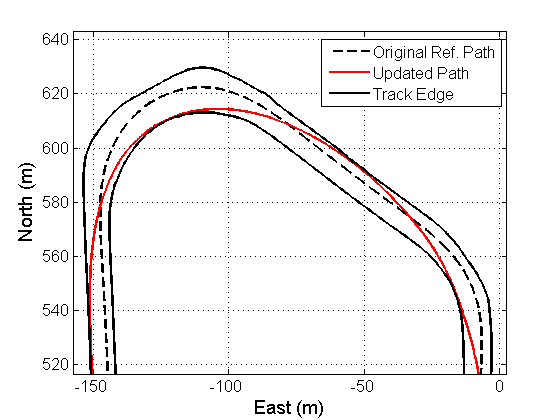
\includegraphics[width=3.25in]{figures/updatedpath.png}
\caption{Path update for an example turn.}
\label{fig:hairpin}
\end{figure}


%%%%%%%%%%%%%%%%%%%%%%%%%%%%%%%%%%%%%%%%%%%%%%%%%%%%%%%%%%%%%%%%%%%%%%
\section*{ALGORITHM IMPLEMENTATION AND RESULTS}
\subsection*{Algorithm Implementation}
The final algorithm for iteratively
generating a vehicle racing trajectory is described in Fig.~\ref{algorithmDesc}. The input to the algorithm is any initial path through the racing circuit, 
parameterized in terms of distance along the path $s$, path curvature $K(s)$, and the lane edge distances $w_\mathrm{in}(s)$ and 
$w_\mathrm{out}(s)$ described in Fig.~\ref{fig:worldInfo}. Given the initial path, the minimum time speed profile $U_x(s)$ is calculated as described in 
Fig.~\ref{fig:VPgen}. Next, the path is modified by solving the previously described minimum curvature
 convex optimization problem (\ref{eq:OPT}). 
 
The optimization only solves explicitly for the steering input $\delta^\star$ and resulting vehicle lateral states $x^\star$ at every 
time step. Included within $x^\star$  is the optimal vehicle heading $\Psi^\star$ and lateral deviation $e^\star$ from the initial path. (Note that $\star$ here refers to an optimal variable assignment, not to be confused with the notation in (\ref{eq:fiala})). To obtain 
the new path in terms of $s$ and $K$, the East-North coordinates ($E_k$, $N_k$) of the updated vehicle path are updated as follows:
 	
\begin{subequations}
%\label{eq:cts}
\begin{align}
	E_k &\gets E_k - e^\star_k\cos(\Psi_{\mathrm{r},k})\\
	N_k &\gets N_k - e^\star_k\sin(\Psi_{\mathrm{r},k})
\end{align}
\end{subequations}
where $\Psi_\mathrm{r}$ is the path heading angle of the original path. Next, the new path is given by the following numerical approximation:
 
 \begin{subequations}
%\label{eq:cts}
\begin{align}
	s_k &= s_{k-1} + \sqrt{(E_k - E_{k-1})^2 + (N_k - N_{k-1})^2}\\ \label{eq:pupdate}
	K_k &= \frac{\Psi^\star_k - \Psi^\star_{k-1}}{s_k - s_{k-1}}
\end{align}
\end{subequations}
  
 Notice that (\ref{eq:pupdate}) accounts for the change in the total path length that occurs when the vehicle deviates from the original path.
 In addition to $s$ and $K$, the lateral distances to the track edges $w_\mathrm{in}$ and $w_\mathrm{out}$ are different for the new path
 as well, and are recomputed using the Cartesian coordinates for
the inner and outer track edges and ($E_k$, $N_k$). The two-step procedure is iterated until the change in lap time $\Delta t^\star$ from the prior iteration is greater than a small positive 
constant $\epsilon$. Note that a positive value of $\Delta t^\star$ indicates the current iteration
yields a slower lap time compared to the prior iteration. Recall that this is possible given that we have no guarantees of convergence, and that the minimum curvature
solution is not necessarily the minimum time solution.

\begin{figure}
\begin{algorithmic}[1]
\Procedure{GenerateTrajectory}{$s^0, K^0, w_\mathrm{in}^0, w_\mathrm{out}^0$}
\State $\mathrm{path}\gets (s^0, K^0, w_\mathrm{in}^0, w_\mathrm{out}^0)$
\While{$\Delta t^\star < \epsilon$}
\State $U_x \gets \mathrm{calculateSpeedProfile(path)}$
\State $\mathrm{path} \gets \mathrm{minimizeCurvature}(U_x, \mathrm{path})$
\State $t^\star \gets \mathrm{calculateLapTime}(U_x,\mathrm{path})$
\EndWhile
\State \textbf{return} $\mathrm{path},U_x$
\EndProcedure
\end{algorithmic}
\caption{Iterative algorithm for fast generation of vehicle trajectories. Each iteration consists of a sequential two-step approach where
the velocity profile is generated given a fixed path and then the path is updated based on the solution from a convex optimization problem.}\label{algorithmDesc}
\end{figure}
\subsection*{Algorithm Validation}
The proposed algorithm is tested on the 5 km Thunderhill racing circuit in Willows, California, USA. The vehicle parameters 
used for the lap time optimization come from an Audi TTS experimental race vehicle, with relevant parameters shown in Table 1.
 The initial path is obtained by collecting GPS data of the inner and outer track edges and estimating the ($s, K, w_\mathrm{in}, w_\mathrm{out}$)
 parametrization of the track centerline.
 
The algorithm is implemented in MATLAB, with the minimum curvature optimization problem (\ref{eq:OPT}) solved using the CVX software package \cite{boydcvx}. For
the purpose of simplicity, topography effects such as bank and grade were neglected. 

\begin{table}[h]
\footnotesize
\begin{center}
\caption{Optimization Parameters}\label{tb:params}
\begin{tabular}{lccc}
Parameter & Symbol & Value & Units \\\hline
Vehicle mass & $m$ & 1500 & kg \\
Yaw Inertia & $I_z$ & 2250 & $\mathrm{kg \cdot m}^2$\\
Front axle to CG & $a$ & 1.04 & m\\
Rear axle to CG & $b$ & 1.42 & m\\
Front cornering stiffness & $\mathrm{C}_\mathrm{F}$ & 160 & $\mathrm{kN \cdot rad}^{-1}$ \\
Rear cornering stiffness & $\mathrm{C}_\mathrm{R}$ & 180 & $\mathrm{kN \cdot rad}^{-1}$ \\
Friction Coefficient     & $\mu $                  &  0.95 & $\mathrm{-} $ \\
Path Discretization      & $\Delta s$              & 2.75 & $m$\\
Optimization Time Steps  & $T       $              & 1843 & -  \\
Max Engine Force         & -                       & 3750 & N\\\hline
\end{tabular}
\end{center}
\end{table}

\begin{figure}
\centering
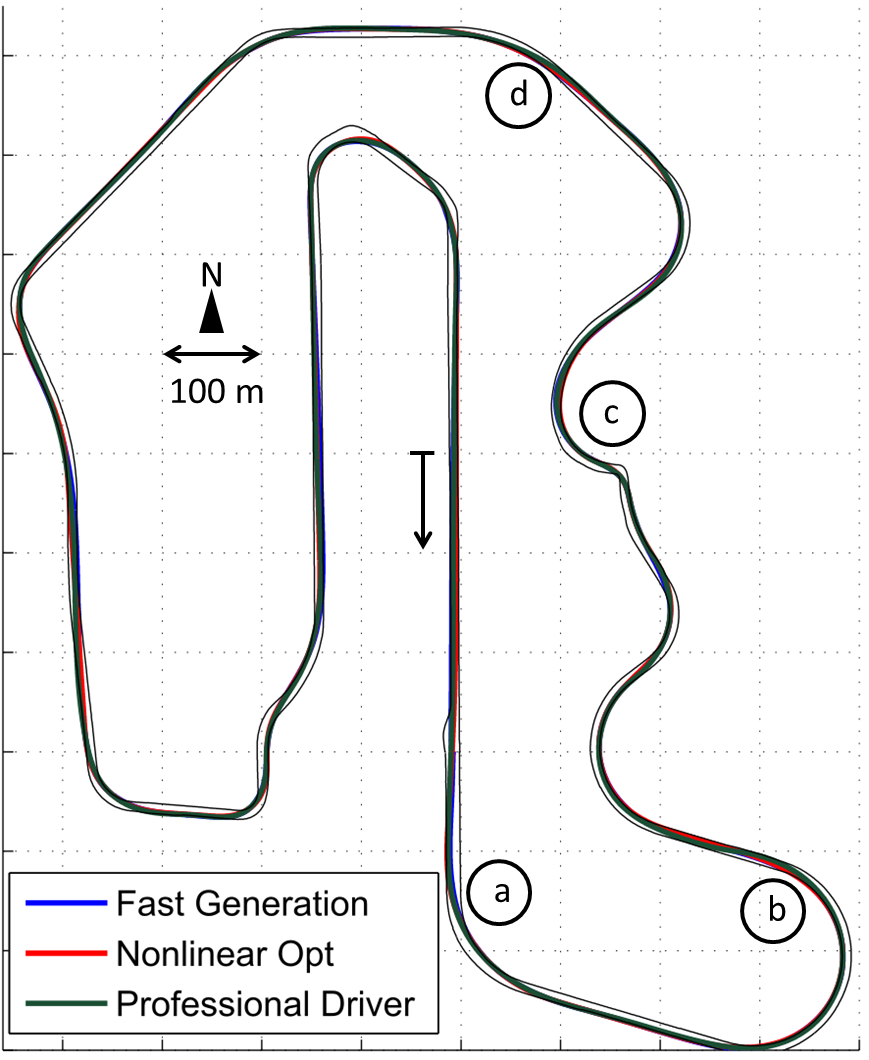
\includegraphics[width=3.3in]{figures/racinglines.png}
\caption{Overhead view of Thunderhill Raceway park along with generated path from algorithm. Car drives in indicated direction around the closed circuit. Labeled regions a-d will be discussed in more detail.}
\label{racingLines}
\end{figure}
\subsection*{Comparison with Other Methods}
The generated racing path after four iterations is shown in
Fig.~\ref{racingLines}. To validate the proposed algorithm, the racing line is compared with results from a nonlinear gradient descent algorithm implemented by 
Theodosis and Gerdes \cite{theodosis} and an experimental trajectory recorded from a professional racecar driver.
 While time-intensive to compute, the gradient descent approach generates racing lines with autonomously driven lap times within one second of
lap times measured from professional racecar drivers. 

\begin{figure}
\centering
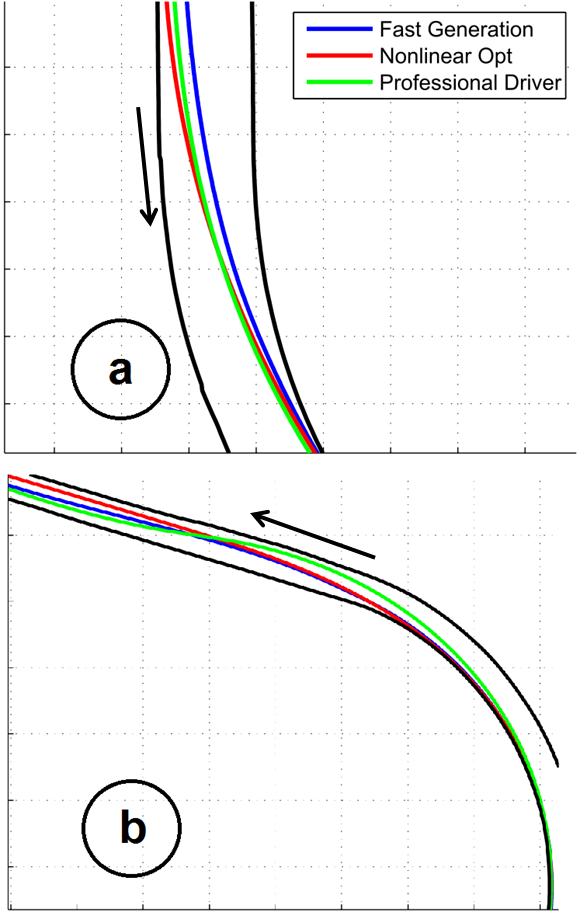
\includegraphics[width=3.5in]{figures/composite1.png}
\caption{Racing lines from the two-step fast generation approach, nonlinear gradient descent algorithm, and experimental data taken
from professional driver. Arrows indicate direction of path. Labeled regions a-b correspond to zoomed-in locations on Fig.~\ref{racingLines}. }
\label{compositeFig1}
\end{figure}

In general, the two-step method provides a racing line that is very similar to the line from the gradient descent method
and the human experimental data. However, several interesting discrepancies are plotted
in Fig.~\ref{compositeFig1} and Fig.~\ref{compositeFig2} for zoomed-in portions of the race track. The discrepancies arise because the nonlinear method balances the tradeoff between a minimum curvature path and the path with shortest total distance,
and finds regions where it may be beneficial to use less of the available road width or drive a higher curvature path in order to reduce the total distance
traveled. However, like most nonlinear racing line optimization techniques, the method in \cite{theodosis} is only guaranteed
to converge to a locally minimal solution. Interestingly, in both \circled{b} and \circled{c}, the
two-step method provides a closer match to the professional driver, while the gradient descent solution matches the professional driver better in \circled{a}. 
For the case of \circled{d}, both numerical methods provide similar results, but this result is different from the path chosen by the human driver.



\begin{figure}
\centering
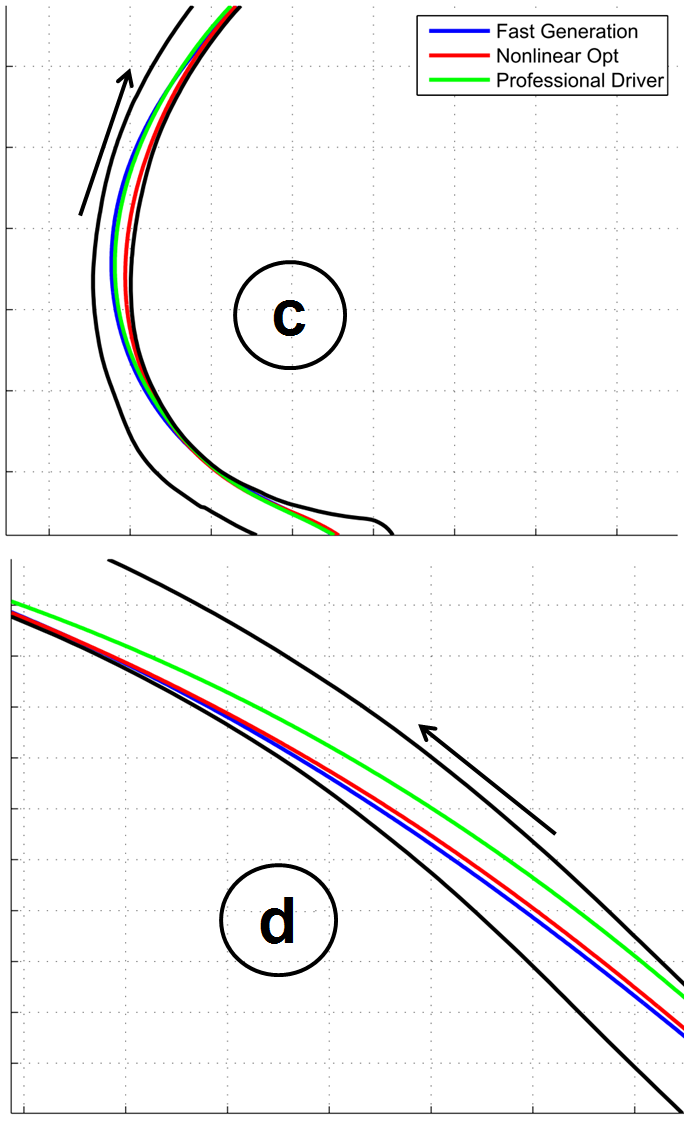
\includegraphics[width=3.5in]{figures/composite2.png}
\caption{Racing lines from the two-step fast generation approach, nonlinear gradient descent algorithm, and experimental data taken
from professional driver. Arrows indicate direction of path. Labeled regions c-d correspond to zoomed-in locations on Fig.~\ref{racingLines}. }
\label{compositeFig2}
\end{figure}

\begin{figure}
\centering
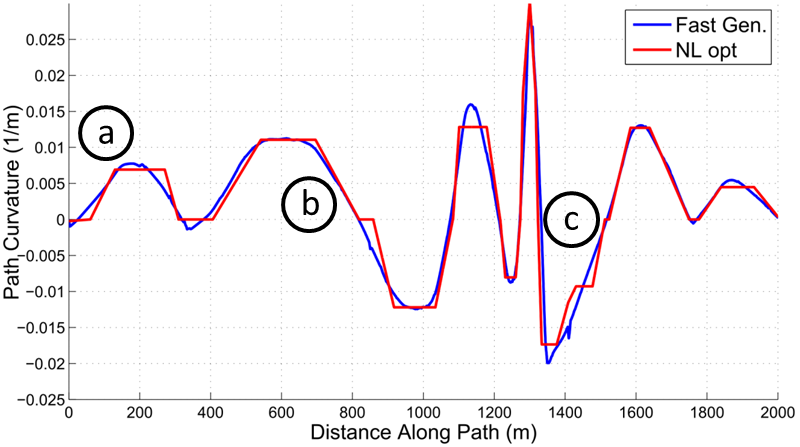
\includegraphics[width=3.5in]{figures/curvatureprofiles.png}
\caption{Curvature profile $K(s)$ plotted vs. distance along the path $s$. For improved visibility, results
 are shown for the first 2 km of the track.}
\label{kProfiles}
\end{figure}

\begin{figure}
\centering
\includegraphics[width=3.5in]{figures/velocityProfiles.png}
\caption{Velocity profile $U_x(s)$ plotted vs. distance along the path $s$ for the two-step method and nonlinear
gradient descent method.}
\label{UxProfiles}
\end{figure}

To further compare the path generation methods, Fig.~\ref{kProfiles} shows the path curvature profile $K(s)$ for both algorithms.
Again, the curvature profiles look similar, with small discrepancies around $s = 900$m, $s = 1100$m and $s=1400$m. The piecewise linear nature of the 
nonlinear gradient descent method is due to the clothoid constraint imposed by \cite{theodosis}. The resulting velocity profiles are 
shown in Fig.~\ref{UxProfiles} for the two-step method and gradient descent method. Interestingly, the gradient descent method is able to achieve higher cornering speeds, although the two-step method
is able to gain a speed advantage by having the vehicle accelerate earlier after a turn is finished.    

\subsection*{Lap Time Convergence and Computation Time}

Fig.~\ref{lapTimes} shows the predicted lap time for each iteration of the two-step algorithm, with step 0 corresponding
to the race track centerline.  While the lap time can be estimated by (\ref{integrateEq}), we 
obtained a more precise lap time by numerically simulating a vehicle following the desired path and velocity profile using the feedback-feedforward control formulation
presented in \cite{mickgeneral}. The equations of motion are the nonlinear versions of (\ref{eq:bm}) with tire forces given by
the brush tire model in (\ref{eq:fiala}). The benefit of using the more precise lap time simulation is accounting for the path tracking dynamics
 of the vehicle and ensuring the car actually stays on the track at all times when subjected to a more accurate vehicle dynamics model. 
 After three iterations, the predicted lap time achieves a minimum value of 135.0 seconds. The predicted lap time
on the fourth iteration degrades slightly to 135.3 seconds, at which the algorithm terminates. The minimum lap time is similar 
to the predicted lap time of 135.5 seconds from the nonlinear gradient descent approach, 
although in reality, the actual experimental lap time achieved  will depend significantly on factors such 
as three-dimensional path topography and engine dynamics.  

\begin{figure}
\centering
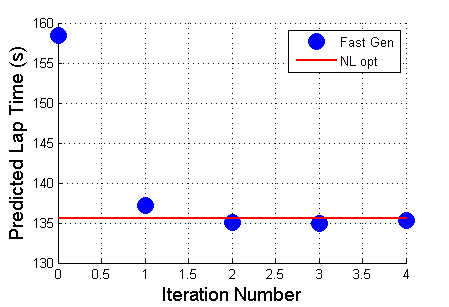
\includegraphics[width=3in]{figures/laptimes.png}
\caption{Lap time as a function of iteration for the two-step fast trajectory generation method. Final lap time is comparable
to that achieved with the nonlinear gradient descent approach. Iteration zero corresponds to the lap time for driving the initial path.}
\label{lapTimes}
\end{figure}

The primary benefit of the proposed algorithm is not improved lap time performance
over the nonlinear algorithm but rather a radical improvement in computational simplicity and speed. Each two-step iteration of the full
course takes only 26 seconds on an Intel i7 processor, whereas the nonlinear algorithm from \cite{theodosis} typically runs over the course of several hours on the same
machine. The most significant computational expense for the proposed algorithm is solving the convex curvature minimization problem for all 1843 discrete time steps of the race vehicle over the 5 km racing circuit.
This computational efficiency will enable future work to incorporate the trajectory modification algorithm as an online ``preview" path planner, which would 
provide the desired vehicle trajectory for an upcoming portion of the race track. Since the computation time of the
 algorithm is heavily dependent on the preview distance, the high-level planner would not need to run at the
 same sample time as the vehicle controller. Instead, the planner would operate on a separate CPU and provide a velocity profile and racing line for only
 the next 1-2 kilometers of the race track every 5-10 seconds, while incorporating estimates of the friction coefficient and other vehicle parameters learned over
 several laps of racing. 

%%%%%%%%%%%%%%%%%%%%%%%%%%%%%%%%%%%%%%%%%%%%%%%%%%%%%%%%%%%%%%%%%%%%%%
\section*{CONCLUSION}

This paper demonstrates an iterative algorithm for quickly generating vehicle racing trajectories, where each iteration is comprised of
 a sequential velocity update and path update step. Given an initial path through the race track, the 
 velocity update step performs forward-backward integration to determine the minimum time speed inputs. Holding this speed 
 profile constant, the path geometry is updated by solving a convex optimization problem to minimize path curvature. The trajectory
 generated by the algorithm for the Thunderhill Raceway circuit is comparable to a trajectory 
 from a previously published nonlinear gradient descent algorithm and an experimental trajectory collected from a
 professional driver. Future work will apply the racing trajectory on a vehicle testbed to determine the experimental performance of the algorithm. 
 Finally, an exciting opportunity for future research is incorporating the trajectory modification algorithm into an online path planner to provide preview trajectories in real time. 

\bibliographystyle{asmems4}


%%%%%%%%%%%%%%%%%%%%%%%%%%%%%%%%%%%%%%%%%%%%%%%%%%%%%%%%%%%%%%%%%%%%%%
\begin{acknowledgment}
The authors would like to thank Marcial Hernandez for assistance with fitting an initial curvature profile from GPS point cloud data, as well as
Vincent Laurense, John Kegelman and Ohi Dibua of the Dynamic Design Laboratory. Kapania and Subosits are both supported by Stanford Graduate Fellowships. 
\end{acknowledgment}


\bibliography{dscc2015}

\end{document}
